\usepackage{xcolor}
\usepackage{afterpage}
\usepackage{pifont,mdframed}
\usepackage[bottom]{footmisc}
\usepackage{minted}

\createsection{\Grader}{Grader di prova}
\newcommand{\inputfile}{\texttt{stdin}}
\newcommand{\outputfile}{\texttt{stdout}}
\makeatletter
\renewcommand{\this@inputfilename}{\texttt{stdin}}
\renewcommand{\this@outputfilename}{\texttt{stdout}}
\renewcommand{\this@syllabuslevel}{5}
\renewcommand{\this@custdifficulty}{3}
\makeatother
\setdifficulty{4}

% % % % % % % % % % % % % % % % % % % % % % % % % % % % % % % % % % % % % % % % % % %
% % % % % % % % % % % % % % % % % % % % % % % % % % % % % % % % % % % % % % % % % % %
Carlo e Alice stanno organizzando le loro vacanze estive e hanno intenzione di prendere una serie di $N-1$ voli.
Gli aeroporti sono identificati da un numero intero univoco.

\begin{figure}[h]
    \centering
    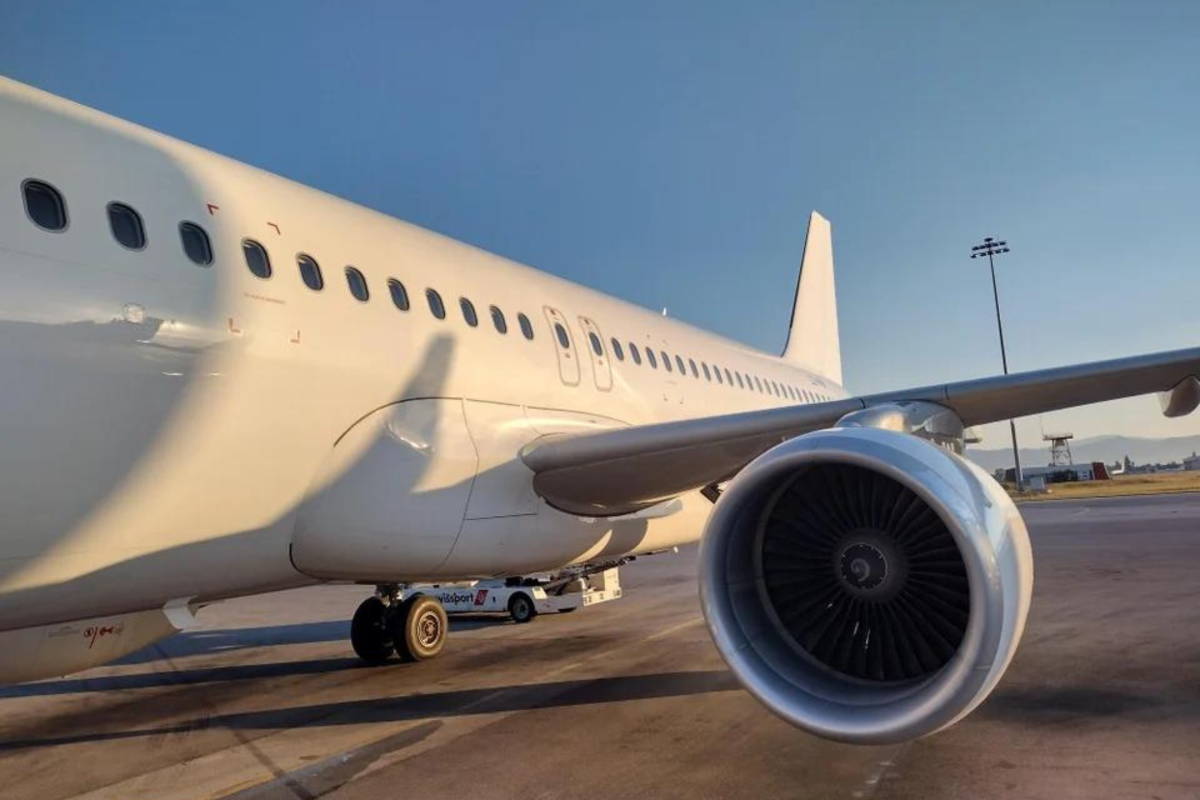
\includegraphics[width=0.4\textwidth]{./plane.png}
    \caption{L'aereo che prenderanno quest'estate.}
\end{figure}

Partiranno dall'aeroporto $A_0$ e prenderanno un volo per l'aeroporto $A_1$, poi un volo da $A_1$ a $A_2$ e così
via fino all'aeroporto $A_{N-1}$.

Ad Alice piace molto prendere l'aereo, ed ha una sequenza di $L-1$ voli che la affascina particolarmente.
Le piace partire dall'aeroporto $B_0$ e andare all'aeroporto $B_1$, poi da $B_1$ a $B_2$ e così via fino a $B_{L-1}$.

Trova quante volte la sequenza di voli preferita da Alice viene percorsa nelle vacanze organizzate.

\Implementation

Dovrai sottoporre un unico file, con estensione \texttt{.cpp}.

\begin{warning}
    Tra gli allegati a questo task troverai un template \texttt{route.cpp} con un esempio di implementazione.
\end{warning}

Il file di input è composto da $3$ righe:
\begin{itemize}
    \item Riga 1: l'intero $N$ e $L$, separati da uno spazio.
    \item Riga 2: $N$ interi che compongo l'array $A$.
    \item Riga 3: $L$ interi che compongo l'array $B$.
\end{itemize}

Il file di output è composto da $1$ riga:
\begin{itemize}
    \item Riga 1: la risposta al problema.
\end{itemize}

% % % % % % % % % % % % % % % % % % % % % % % % % % % % % % % % % % % % % % % % % % %
% % % % % % % % % % % % % % % % % % % % % % % % % % % % % % % % % % % % % % % % % % %

\Constraints

\begin{itemize}[nolistsep, itemsep=2mm]
    \item $2 \le N \le 1\:000\:000$.
    \item $2 \le L \le N$.
    \item $0\le A_i \le 10^6$ per ogni $i = 0 \dots N-1$.
    \item $0 \le B_i \le 10^6$ per ogni $i = 0 \dots M-1$.
    \item L'array $A$ e $B$ possono contenere più volte lo stesso aeroporto.
    \item Possono esistere voli panoramici, ovvero voli che partono e atterrano nello stesso aeroporto.
\end{itemize}

% % % % % % % % % % % % % % % % % % % % % % % % % % % % % % % % % % % % % % % % % % %
% % % % % % % % % % % % % % % % % % % % % % % % % % % % % % % % % % % % % % % % % % %

\Scoring

Il tuo programma verrà testato su diversi test case raggruppati in subtask.
Per ottenere il punteggio relativo ad un subtask,
è necessario risolvere correttamente tutti i test che lo compongono.

\IIOTsubtask{0}{1}{Casi d'esempio.}

\IIOTsubtask{16}{1}{$L = 2$}

\IIOTsubtask{23}{2}{$N \le 1000$}

\IIOTsubtask{38}{2}{$N \cdot L \le 1\:000\:000$}

\IIOTsubtask{23}{3}{Nessuna limitazione aggiuntiva.}



% % % % % % % % % % % % % % % % % % % % % % % % % % % % % % % % % % % % % % % % % % %
% % % % % % % % % % % % % % % % % % % % % % % % % % % % % % % % % % % % % % % % % % %

\Examples

\begin{example}
    \exmpfile{route.input0.txt}{route.output0.txt}%
    \exmpfile{route.input1.txt}{route.output1.txt}%
\end{example}

% % % % % % % % % % % % % % % % % % % % % % % % % % % % % % % % % % % % % % % % % % %
% % % % % % % % % % % % % % % % % % % % % % % % % % % % % % % % % % % % % % % % % % %

\Explanation

Nel primo caso d'esempio, la sequenza di aeroporti $2 \rightarrow 3 \rightarrow 4$ viene visitata una volta sola.

Nel secondo caso d'esempio, Alice e carlo compiono diversi voli panoramici ($0 \rightarrow 0$).
Ci sono $3$ sequenze di aeroporti preferite da Alice.